\begin{titlepage}
\null\vskip-47pt
\hbox to \textwidth
{\bf [Per \holn{} \holnversion] { \hfil \today}}

\setcounter{page}{1}                      % titlepage IS page 1

\vspace*{60mm}


{\fontfamily{ptm}\selectfont
\begin{center}
\scalebox{1.4}{\begin{tabular}{c} \Huge TUTORIAL \\[4pt] \huge del Sistema HOL \end{tabular}} \\
\end{center}}

\begin{center}
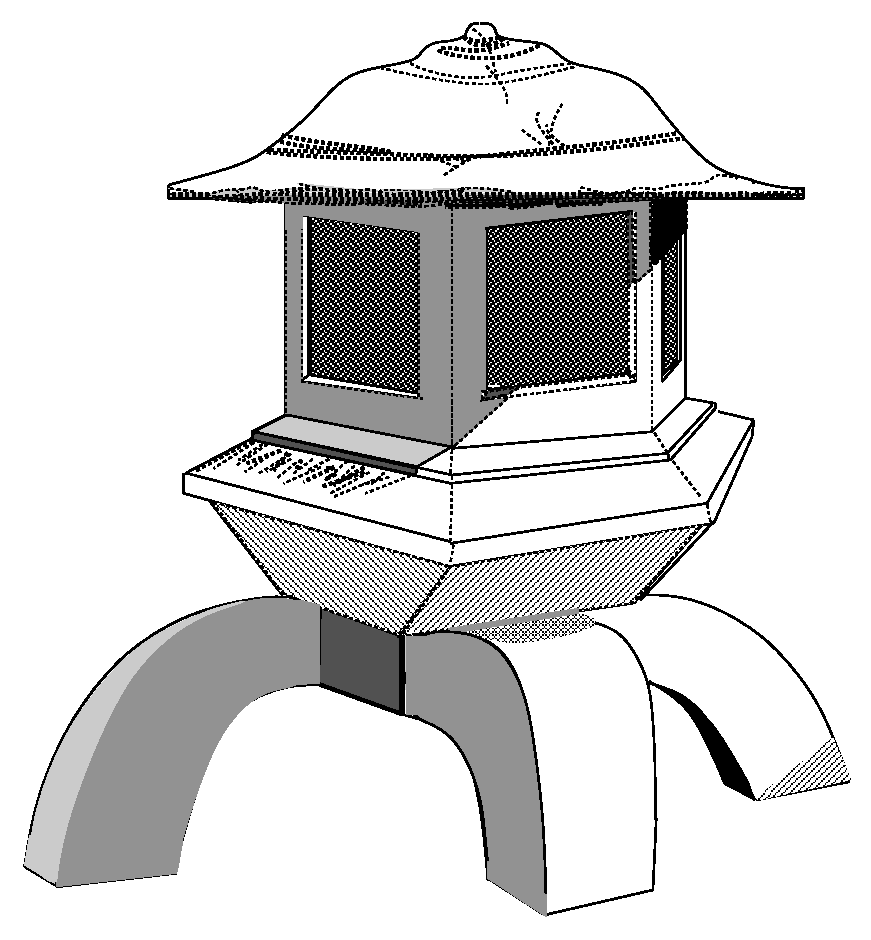
\includegraphics[width=3.8cm]{../../../Logo/lantern}
\end{center}


\vfill
\end{titlepage}

% To kick a blank page with no header
\thispagestyle{empty}
\cleardoublepage

%END LATEX

%HEVEA \begin{tabular}{l@{\hspace{5cm}}r}
%HEVEA {\bf [For \holn{} \holnversion]} & \today\\
%HEVEA \end{tabular}
%HEVEA
%HEVEA \begin{center}
%HEVEA {\Huge\bf The HOL System}\\
%HEVEA {\LARGE \bf TUTORIAL}\\
%HEVEA \vspace{1cm}
%HEVEA \begin{toimage}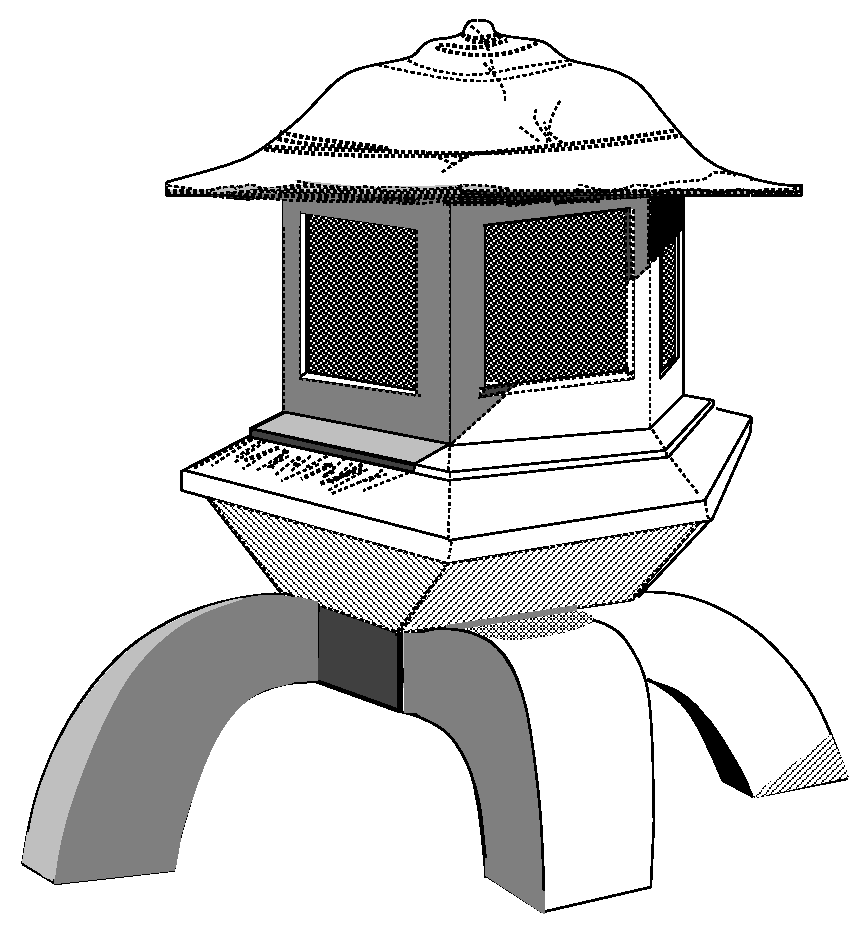
\epsfig{file=../Covers/LANTERN.ps,height=2.5in}\\
%HEVEA \end{toimage}\imageflush
%HEVEA \begin{tabular}{ccc}
%HEVEA University of Cambridge & \hspace*{10ex}DSTO\hspace*{10ex} & SRI International
%HEVEA \end{tabular}
%HEVEA \end{center}




%%% Local Variables:
%%% mode: latex
%%% TeX-master: "tutorial"
%%% End:
